\documentclass{mimosis}

\usepackage{metalogo}

%%%%%%%%%%%%%%%%%%%%%%%%%%%%%%%%%%%%%%%%%%%%%%%%%%%%%%%%%%%%%%%%%%%%%%%%
% Some of my favourite personal adjustments
%%%%%%%%%%%%%%%%%%%%%%%%%%%%%%%%%%%%%%%%%%%%%%%%%%%%%%%%%%%%%%%%%%%%%%%%
%
% These are the adjustments that I consider necessary for typesetting
% a nice thesis. However, they are *not* included in the template, as
% I do not want to force you to use them.

% This ensures that I am able to typeset bold font in table while still aligning the numbers
% correctly.
\usepackage{etoolbox}

%%%%%%%%%%%%%%%%%%%%%%%%%%%%%%%%%%%%%%%%%%%%%%%%%%%%%%%%%%%%%%%%%%%%%%%%
% Hyperlinks & bookmarks
%%%%%%%%%%%%%%%%%%%%%%%%%%%%%%%%%%%%%%%%%%%%%%%%%%%%%%%%%%%%%%%%%%%%%%%%

\usepackage[%
  colorlinks = true,
  citecolor  = RoyalBlue,
  linkcolor  = RoyalBlue,
  urlcolor   = RoyalBlue,
  unicode,
  ]{hyperref}

\usepackage{bookmark}

%%%%%%%%%%%%%%%%%%%%%%%%%%%%%%%%%%%%%%%%%%%%%%%%%%%%%%%%%%%%%%%%%%%%%%%%
% Bibliography
%%%%%%%%%%%%%%%%%%%%%%%%%%%%%%%%%%%%%%%%%%%%%%%%%%%%%%%%%%%%%%%%%%%%%%%%
%
% I like the bibliography to be extremely plain, showing only a numeric
% identifier and citing everything in simple brackets. The first names,
% if present, will be initialized. DOIs and URLs will be preserved.

\usepackage[%
  autocite     = plain,
  backend      = biber,
  doi          = true,
  url          = true,
  giveninits   = true,
  hyperref     = true,
  maxbibnames  = 99,
  maxcitenames = 99,
  sortcites    = true,
  style        = numeric,
  ]{biblatex}

\input{bibliography-mimosis}
\addbibresource{Thesis.bib}

\usepackage{wrapfig}
\usepackage[inline]{enumitem}

\setcapindent{0pt}
\setlength{\intextsep}{0pt}

\usepackage{xr}
\usepackage{amsmath}
\usepackage{gensymb}

\DeclareMathOperator{\atantwo}{atan2}

\DeclareMathOperator{\arctantwo}{arctan2}


\usepackage[vlined,linesnumbered]{algorithm2e}

%%%%%%%%%%%%%%%%%%%%%%%%%%%%%%%%%%%%%%%%%%%%%%%%%%%%%%%%%%%%%%%%%%%%%%%%
% Fonts
%%%%%%%%%%%%%%%%%%%%%%%%%%%%%%%%%%%%%%%%%%%%%%%%%%%%%%%%%%%%%%%%%%%%%%%%

\ifxetexorluatex
  \usepackage{unicode-math}
  \setmainfont{EB Garamond}
  \setmathfont{Garamond Math}
  \setmonofont[Scale=MatchLowercase]{Source Code Pro}
\else
  \usepackage[lf]{ebgaramond}
  \usepackage[oldstyle,scale=0.7]{sourcecodepro}
  \singlespacing
\fi

% \newacronym[description={Principal component analysis}]{PCA}{PCA}{principal component analysis}
% \newacronym                                            {SNF}{SNF}{Smith normal form}
% \newacronym[description={Topological data analysis}]   {TDA}{TDA}{topological data analysis}

% \newglossaryentry{LaTeX}{%
%   name        = {\LaTeX},
%   description = {A document preparation system},
%   sort        = {LaTeX},
% }

% \newglossaryentry{Real numbers}{%
%   name        = {$\real$},
%   description = {The set of real numbers},
%   sort        = {Real numbers},
% }

\makeindex
\makeglossaries

%%%%%%%%%%%%%%%%%%%%%%%%%%%%%%%%%%%%%%%%%%%%%%%%%%%%%%%%%%%%%%%%%%%%%%%%
% Ordinals
%%%%%%%%%%%%%%%%%%%%%%%%%%%%%%%%%%%%%%%%%%%%%%%%%%%%%%%%%%%%%%%%%%%%%%%%

\makeatletter
\@ifundefined{st}{%
  \newcommand{\st}{\textsuperscript{\textup{st}}\xspace}
}{}
\@ifundefined{rd}{%
  \newcommand{\rd}{\textsuperscript{\textup{rd}}\xspace}
}{}
\@ifundefined{nd}{%
  \newcommand{\nd}{\textsuperscript{\textup{nd}}\xspace}
}{}
\makeatother

\renewcommand{\th}{\textsuperscript{\textup{th}}\xspace}

%%%%%%%%%%%%%%%%%%%%%%%%%%%%%%%%%%%%%%%%%%%%%%%%%%%%%%%%%%%%%%%%%%%%%%%%
% Incipit
%%%%%%%%%%%%%%%%%%%%%%%%%%%%%%%%%%%%%%%%%%%%%%%%%%%%%%%%%%%%%%%%%%%%%%%%

\title{Trajectory Control for High-DoF Manipulators}
\subtitle{In an environment filled with obstacles}
\author{Patrick Ondika}

\begin{document}

\frontmatter
  \begin{titlepage}
  \vspace*{5cm}
  \makeatletter
  \begin{center}
    \begin{Huge}
      \@title
    \end{Huge}\\[0.1cm]
    %
    \begin{Large}
      \@subtitle
    \end{Large}\\
    %
    \emph{by}\\
    \@author\\
    %
    \hfill
    \begin{figure}[h]
      \centering
      \includegraphics[width=0.4\textwidth]{fithesis-fi.pdf}
    \end{figure}

    \vfill
    \emph{Master's thesis}\\
    at\\
    \textsc{Masaryk University, Faculty of Computer Science}
  \end{center}
  \makeatother
\end{titlepage}

\newpage
\null
\thispagestyle{empty}
\newpage

  \begin{center}
  \textsc{Declaration}
\end{center}

\noindent

I hereby declare that this paper is my original authorial work, which
I have worked out on my own. All sources, references, and literature
used or excerpted during elaboration of this work are properly cited
and listed in complete reference to the due source.

\hspace*{\fill} Patrick Ondika

\newpage

\begin{center}
  \textsc{Acknowledgements}
\end{center}

\noindent

First and foremost, I'd like to thank Jan Mrázek, for creating the RoFI project, supporting me, and serving as a mentor. His encouragement and willingness to help have been very helpful throughout my entire time in the RoFI project. I'd also like to thank my advisor, Jiřík, for giving me feedback on my work and showing me that you can be successful without abandonning your inner 12-year old. The list goes on to all the other amazing people I met at the faculty; tutors and classmates that, often indirectly, gave me someone to look up to and the motivation to chase after them.

\newpage

\begin{center}
  \textsc{Abstract}
\end{center}
%
\noindent
%
RoFI is a platform of metamorphic robots -- robots consisting of individual modules which each work autonomously and have their own simple joints, but can connect to each other and complete more complex tasks. A natural shape for these robots to take is a robotic arm, which can manipulate with the surrounding objects. What separates RoFI arms from pre-built industrial arms is the total number of joints (degrees of freedom), which rises with each module.

An essential task for robotic arms (manipulators) is the act of moving one object from one place to the other. To successfully accomplish this task, we need to plan a trajectory the manipulator can take to reach the object, while avoiding collisions with potential obstacles. Various algorithms for this problem exist, but the complexity of standard methods scales exponentially with each degree of freedom, making them unusable for RoFI arms.

This thesis aims to design and implement an algorithm for trajectory planning of robotic manipulators with a very high degree of freedom. The thesis goes through the process of designing such an algorithm, explains the individual components, and presents the algorithm as a whole. Finally, the results are evaluated in a simulator within the RoFI environment.

\vfill
Keywords: RoFI, Metamorphic robots, Modular robots, Inverse kinematics, FABRIK, Motion planning, Path planning, Robotic manipulator


  \tableofcontents

\mainmatter

  % \part[A good part]{%
  %   A good part\\
  %   %
  %   \vspace{1cm}
  %   %
  %   \begin{minipage}[l]{\textwidth}
  %   %
  %   \textnormal{%
  %     \normalsize
  %     %
  %     \begin{singlespace*}
  %       \onehalfspacing
  %       %
  %       You can also use parts in order to partition your great work
  %       into larger `chunks'. This involves some manual adjustments in
  %       terms of the layout, though.
  %     \end{singlespace*}
  %   }
  %   \end{minipage}
  % }

  %%%%%%%%%%%%%%%%%%%%%%%%%%%%%%%%%%%%%%%%%%%%%%%%%%%%%%%%%%%%%%%%%%%%%%%%
\chapter{Introduction}
%%%%%%%%%%%%%%%%%%%%%%%%%%%%%%%%%%%%%%%%%%%%%%%%%%%%%%%%%%%%%%%%%%%%%%%%


In a world of automation, we would like to tell our robots a task such
as \enquote{Hand me a coffee.} and expect them to do it without giving
specific instructions of \textit{how} to do it.

This seemingly basic task contains many interesting subproblems, including but not limited to
the high level design of the robot, hardware design and programming, image or speech recognition, and human computer interaction.
For us, the critical part will be performing the task itself; in this case, computing and realising the movement necessary to grab a cup and deliver it to the target location.

A natural way for us to approach the problem is to create a humanoid robot, or simply a robotic arm on a fixed base. Even if we limit ourselves to the latter, the idea is quite fascinating; outside of making coffee for computer scientists, it can assist engineers or surgeons in their work.

This thesis aims to create a general algorithm for controlling robotic arms.
Our assumption is that we have a robotic arm that is fixed in place and has a high number of joints.
Naturally, the joints on the arm will have limited range, as many real arms do.
The task we are aiming to accomplish is to plan movement of the arm from one place to another, while avoiding collisions with other objects in the workspace of the arm.
The performed movement should be reasonably efficient, and the computation needs to be fast.

The presented methods will not be limited to a specific setup, but the results will be demostrated on top of the RoFI platform\cite{rofiPlatform}.

As computer scientists, we can already sense that we are tackling a rather complex problem, which is yet to be solved by the robotic community. Obstacles and joint constraints generally make the problem of motion planning\footnote{The general problem of computing the motion of a robot. It encompasses robotic arms as well as self driving cars and walking robots.} hard to perform, and the task of finding a good solution often goes directly against the task of finding a solution quickly.
There are many existing attempts to create an algorithm for motion planning of robotic arms,
some of which have been successfully used in practice to perform a specific task. Each method has specific advantages and disadvantages, which will be discussed in further chapters of this thesis.

What mostly sets our goals apart from previous research is the assumption that we have a high number of joints. This fact, at its core, makes traditional methods for related problems computationally infeasible.
Being unable to use a single existing method will lead us to decomposing the problem into smaller parts and combining various algorithms from different areas. By the end, we hope to build a satisfiable solution, starting with each component from the ground up.

Outside of robotics, having a general algorithm with this specification is interesting for computer graphics, in particular for generating character movement in videogames.
With an algorithm that can compute the motion of a constrained limb with a high number of joints at our disposal, we can design complex kinematic models and animate movement of the respective characters in complex environments.

%%%%%%%%%%%%%%%%%%%%%%%%%%%%%%%%%%%%%%%%%%%%%%%%%%%%%%%%%%%%%%%%%%%%%%%%
\section{Outline of the work}
%%%%%%%%%%%%%%%%%%%%%%%%%%%%%%%%%%%%%%%%%%%%%%%%%%%%%%%%%%%%%%%%%%%%%%%%

This thesis will try to lead the reader through the process of designing an algorithm for the motion planning of robotic arms. We will start with a more formal definition of the problem, preliminary knowledge, and introduction of the platform our solution will be presented on.

As we try to incrementally design an algorithm, the discussion of state of the art methods, some mathematical theory, and main ideas behind the implementation will be tied together to create the core of this thesis. Each idea will be accompanied by the intuition behind it, as well as a visual representation. Apart from the ideas that will build our final solution, we will explore methods that were not successful, and discuss the limits of different approaches.

Finally, the solution will be tested and evaluated. We will showcase the behavior of the algorithm in various environments, and present a possible application for it. We will run benchmarks to evaluate the efficiency and success rate of the algorithm. At the end, takeaways from the design process and further improvements will be discussed.

  \chapter{Preliminaries}

To start, we need to establish terminology and preliminary knowledge. Throughout this thesis, we will be discussing robotic arms; in robotic terms, they are more commonly referred to as \textit{manipulators}.

\begin{wrapfigure}{r}{0.25\textwidth}
    \centering
    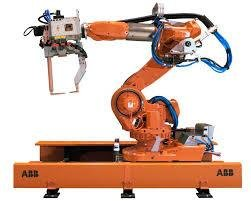
\includegraphics[width=0.35\textwidth]{Industrial-robotic-arm.jpeg}
  \caption{\\Industrial robotic arm with a gripper~\cite{manipulator}}
\end{wrapfigure}


Robotic manipulators are programmable mechanical devices, typically fixed in place. They are responsible for moving objects or tools and performing various tasks. They are widely used in factories for mass production of vehicles, electronics, etc. Based on the equipment of the specific manipulator, it can move objects from one assembly line to another, cut things, or solder parts together. However, such manipulators are often tailored to perform one specific motion repeatedly, thus, they will not be the focus of this work.

Manipulators consist of solid bodies, linked via movable joints. They often resemble human arms, although the specific shapes vary wildly.

We consider 2 basic types of joints, see Figure~\ref{fig:basicjoints}:
\begin{itemize}
  \item Revolute\footnote{Also referred to as rotary or rotational.} joints: the most common type. They consist of a motor rotating the next body around an axis. Depending on the type of motors and the build of the robot, the rotation may either be unbounded, or have a specific range of motion.
  \item Prismatic joints: these perform linear motion along the joint axis.
\end{itemize}

\begin{figure}[h]
\centering
\begin{subfigure}{.5\textwidth}
  \centering
  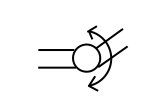
\includegraphics[width=.4\linewidth]{revolute.jpg}
  \caption{Revolute joints perform a rotation along their axis}
\end{subfigure}%
\begin{subfigure}{.5\textwidth}
  \centering
  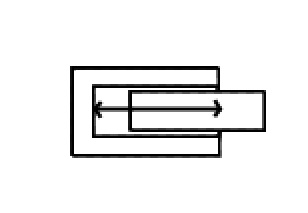
\includegraphics[width=.4\linewidth]{prismatic.png}
  \caption{Prismatic joints perform a linear motion along their axis}
\end{subfigure}
\caption{Basic joint types; the arrow refers to the respective range of motion.}
\label{fig:basicjoints}
\end{figure}

There are joint types that can perform more complicated motion, but they can generally be modelled as a combination of the basic two. Ball joints allow rotation in any direction; in a kinematic system, they can be modelled as two revolute joints in the same place. Cylindrical joints allow for both rotation and extension, serving as a combination of revolute and prismatic joints.

The state of the robot is called its configuration. A configuration is uniquely defined by two things:
\begin{itemize}
  \item The build of the robot: shape of the bodies, how they are connected, and the types of joints.
  \item The parameters of its joints.
\end{itemize}

The number of parameters that define a robotic system is referred to as degrees of freedom (DoF). Revolute and prismatic joints each have one degree of freedom. The parameter of a revolute joint is the current angle of rotation; the parameter of a prismatic joint is the current length it's extended at. Ball and cylindrical joints each have two degrees of freedom, respectively. The DoF of a robotic manipulator is the sum of DoFs of its flexible joints.

The end of a robotic arm is called the end effector. Typically, the end effector is different from the rest of the manipulator; it consists of a tool specialized to the robot's task. The end effector is designed to interact with the robot's environment, and there are many variatons. If the manipulator is designed to move objects, the end effector can be a fingerlike gripper, claw, or even use electromagnetic forces~\cite{grippers}. In handling textile materials, the end effector can be equipped with scissors, pins or needles.

When we refer to the position of the end effector, we mean its location and rotation in cartesian space. The parameter of a joint, such as its current rotation or extension, is sometimes called its position as well; not to be confused with its position in space. Though we will see that generally, knowing the joint parameters will let us compute their position in space, and vice versa.

\section{Kinematics of robotic manipulators}

The science that studies the relationship between joint parameters and the positions in cartesian space -- particularly the end effector -- is called kinematics.
We differentiate between forward and inverse kinematics.

Forward kinematics is the problem of finding the end effector position knowing the joint parameters. For manipulators with traditional joints, solving this problem is simple enough, and there is always a unique solution. The specifics differ based on the build of the robot, but there is a standard convention for it.

A method for computing forward kinematics was published by Denavit and Hartenberg in 1955~\cite{dh} and became the de-facto standard for robotics. The Denavit-Hartenberg (DH) method utilises $4\times4$ matrices to represent affine transformations in homogenous coordinates~\cite{nomizu1994affine}.
These matrices allow an efficient representation of both rotation and translation in 3D space.
In a kinematic system, such as a robot manipulator, each joint has its accompanying transformation matrix, and the position of the end effector is obtained by repeatedly applying the joint transformations through matrix multiplication. The base of the arm is commonly considered the origin of the manipulator's coordinate system, therefore it is simply the identity matrix:

\begin{equation}
  T_0 =  \begin{bmatrix}
            1 & 0 & 0 & 0 \\ 0 & 1 & 0 & 0 \\ 0 & 0 & 1 & 0 \\ 0 & 0 & 0 & 1 \\
          \end{bmatrix}
\end{equation}

Joint transformations are expressed as translations or rotations along the X and Z axes.
Translation along the Z axis is expressed as:

\begin{equation}
  Trans_Z(d) = \begin{bmatrix}
                 1 & 0 & 0 & 0 \\ 0 & 1 & 0 & 0 \\ 0 & 0 & 1 & d \\ 0 & 0 & 0 & 1 \\
               \end{bmatrix}
\end{equation}

Whereas the rotation is expressed as:

\begin{equation}
  Rot_Z(\theta) = \begin{bmatrix}
                    \cos{\theta} & -\sin{\theta} & 0 & 0 \\
                    \sin{\theta} & \cos{\theta} & 0 & 0 \\
                    0 & 0 & 1 & 0 \\ 0 & 0 & 0 & 1 \\
             \end{bmatrix}
\end{equation}

The transformations around the X axis are expressed analogously:

\begin{equation}
  Trans_X(r) = \begin{bmatrix}
                 1 & 0 & 0 & 0 \\ 0 & 1 & 0 & 0 \\ 0 & 0 & 1 & r \\ 0 & 0 & 0 & 1 \\
               \end{bmatrix}
\end{equation}


\begin{equation}
  Rot_X(\alpha) = \begin{bmatrix}
                    1 & 0 & 0 & 0 \\
                    0 & \cos{\alpha} & -\sin{\alpha} & 0 \\
                    0 & \sin{\alpha} & \cos{\alpha} & 0 \\
                    0 & 0 & 0 & 1 \\
             \end{bmatrix}
\end{equation}

Altogether, for a single joint i, we obtain the transformation matrix:

\begin{equation}
  T_i = \begin{bmatrix}
          \cos{\theta_i} & -\sin{\theta_i}\cos{\alpha_i} & \sin{\theta_i}\sin{\alpha_i} & r_i\cos{\theta_i} \\
          \sin{\theta_i} & \cos{\theta_i}\cos{\alpha_i} & -\cos{\theta_i}\sin{\alpha} & r_i\sin{\theta_i} \\
          0 & \sin{\alpha_i} & \cos{\alpha_i} & d_i \\
          0 & 0 & 0 & 1 \\
        \end{bmatrix}
\end{equation}

To obtain the position of the end effector (or any other link) of a manipulator, we simply need to multiply all the joint transformations leading up to it:

\begin{equation}
  [T] = T_0T_1\cdots T_{n-1}T_n
\end{equation}

Notice that each matrix in the Denavit-Hartenberg convention is in form
\[
    T = \begin{bmatrix}
        \begin{array}{c|c}
           \begin{matrix}
              & & & \\
              & & R & & \\
              & & &
           \end{matrix}
            & t \\
        \midrule
        \begin{matrix}
              0 & 0 & 0 \\
           \end{matrix}
            & 1 \\
        \end{array}
    \end{bmatrix}
\]
\noindent where R is the $3\times3$ rotational part of the matrix, which is always orthonormal, and $t$ represents the displacement along the 3 axes. This allows for efficient computation of the inverse, since the inverse of an orthonormal matrix is equal to its transpose, and the inverse of a translation is simply its negation. By multiplying the two inversions, we get:

\[
    T^{-1} = \begin{bmatrix}
        \begin{array}{c|c}
           \begin{matrix}
              & & & \\
              & & R^T & & \\
              & & &
           \end{matrix}
            & -R^{T}t \\
        \midrule
        \begin{matrix}
              0 & 0 & 0 \\
           \end{matrix}
            & 1 \\
        \end{array}
    \end{bmatrix}
\]

Knowing the transformation matrix of a specific joint allows us to easily compute the positions of joints. Knowing the inverse of a joint's transformation matrix allows us to easily compute positions of other objects in the workspace with respect to the joint, which will be useful later on.

Since the movements of traditional joints can easily be represented as a combination of the two rotations and translations, we consider the forward kinematics of robotic manipulators a solved problem.

\newpage

\begin{wrapfigure}{r}{0.25\textwidth}
    \centering
    \begin{minipage}{.25\textwidth}
        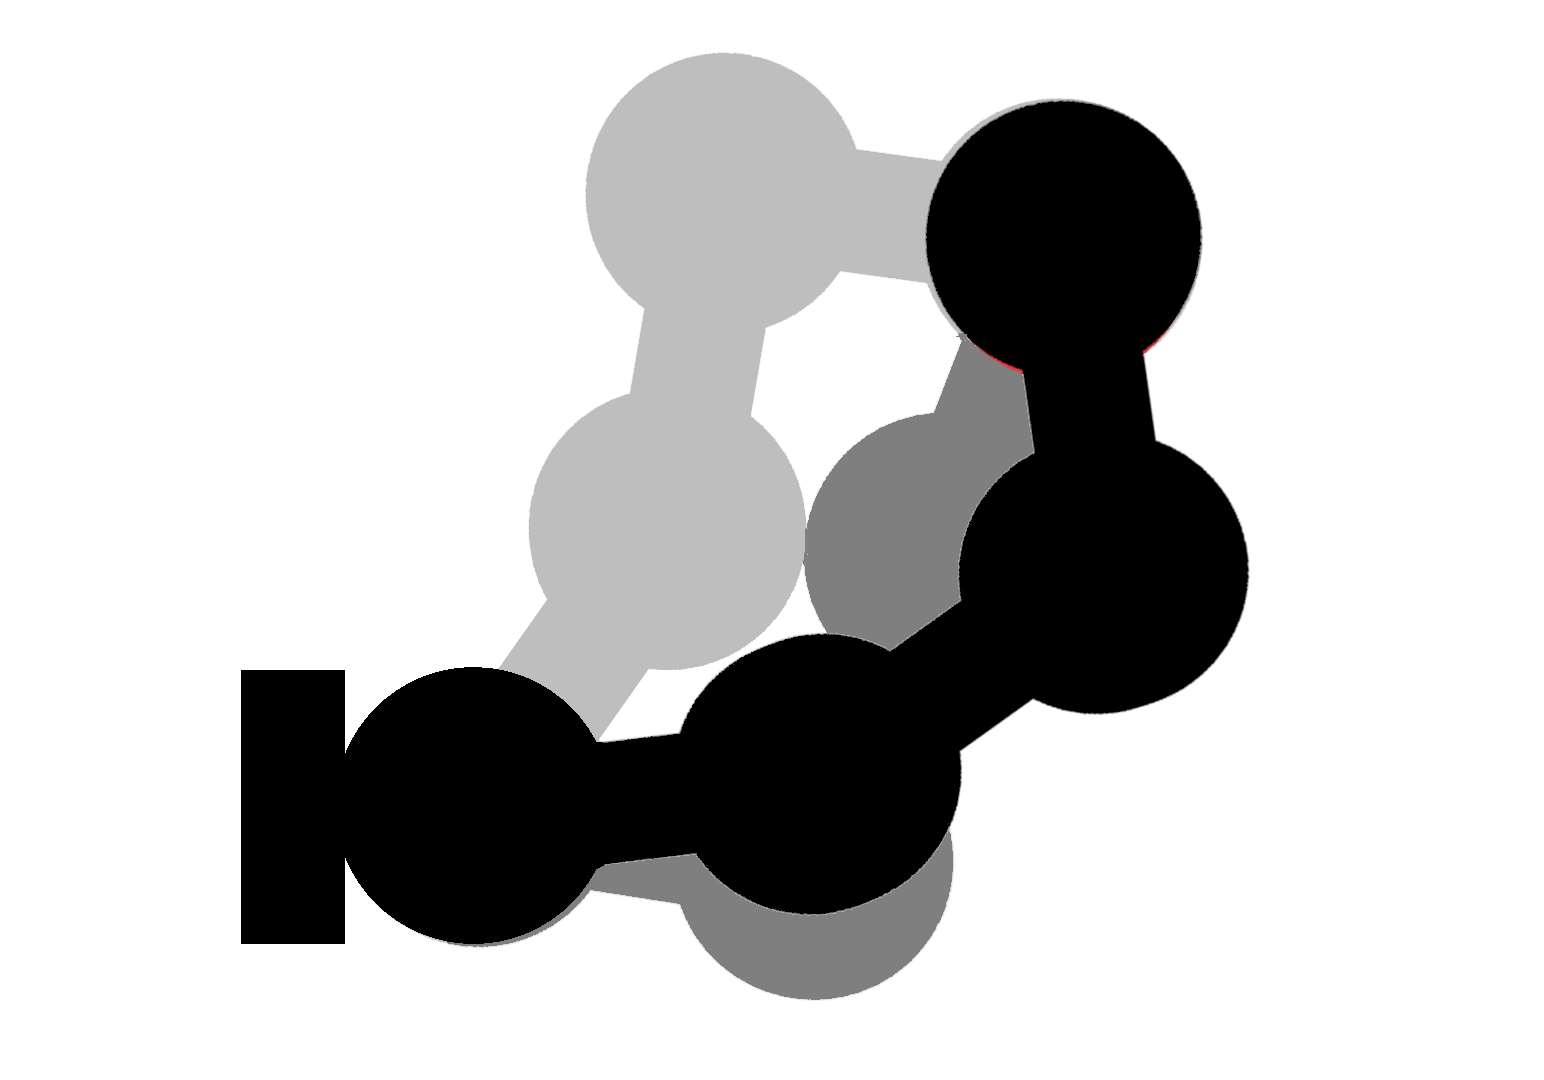
\includegraphics[width=\textwidth]{redundant.png}
    \end{minipage}
    \caption{\\3 example IK solutions to the same problem~\cite{Ondika2021thesis}}\label{fig:redun}
\end{wrapfigure}

Inverse kinematics (IK), as the name suggests, is the inverse to the forward kinematics problem: given a position for the end effector, we wish to compute the corresponding joint parameters. This is a significantly harder problem. If there are exactly as many degrees of freedom in the manipulator as the dimension of the target\footnote{Industrial manipulators commonly have exactly 6 degrees of freedom, which corresponds to a target in cartesian space, consisting of the x-y-z dimensions and a rotation around each of the axes.}, there are ways to obtain an exact analytical solution. However, as we are considering manipulators with a significantly higher DoF, there will generally be an infinite number of solutions (see Figure~\ref{fig:redun}). Hence, numerical methods have to be used.

Common methods for solving inverse kinematics view the problem as an optimization problem, and iteratively try to minimize the distance between the target and the current position of the end effector. All the different methods for inverse kinematics are not the topic of this thesis, and only a short summary will be provided. For a complete overview, see~\cite{overview}.

The methods most discussed in literature are based on approximating the inversion of a Jacobian matrix. For robotic manipulators, the Jacobian matrix is a matrix of partial derivatives at each joint. The size of the matrix is $m \times n$, where $m$ corresponds to the target dimension (6 for the 3D problem of reaching a target) and $n$ corresponds to the degrees of freedom.
The Jacobian matrix provides us with a linear approximation of how the end effector is going to move when slight changes in the joint positions are made. Hence, if we could invert this matrix, we would get an estimation of how to move the joints in order to move the end effector closer to the target. Then, by iteratively repeating this process, we could obtain a solution. However, the Jacobian matrix generally does not have an inversion; the matrix is not square for manipulators with over 6 degrees of freedom, and even then, the determinant is not guaranteed to be nonzero.

There are many methods that try to approximate the inverse, most notably the Moore-Penrose inverse, known as the matrix pseudoinverse~\cite{penrose_1955}. This matrix serves as the generalisation of the matrix inverse, and exists for any matrix. The Jacobian pseudoinverse technique for inverse kinematics was heavily studied, but it suffers from a few fundamental drawbacks. It's hard to incorporate local joint limits, and the method behaves erratically near singularities -- a state where the manipulator is straightened out and slight movement of any joint results in roughly the same change.
In addition to that, it is not very efficient, as the Jacobian matrix and its pseudoinverse have to be computed repeatedly in each iteration. A common way to compute the pseudoinverse is using Singular Value Decomposition; the complexity of this method is $\mathcal{O}(mn^2)$~\cite{trefethen1997numerical}, which scales poorly with respect to the degrees of freedom.

Some authors~\cite{Wolovich1984ACT} suggest using the transpose of the Jacobian matrix, rather than the pseudoinverse. This method is faster but less precise, and suffers from many of the same problems. There are many modifications and extensions of these algorithms, but since we are considering high-DoF manipulators, they are not as interesting for us.

The other branch of inverse kinematics algorithms are heuristic techniques. These consist of simpler computations and make decisions locally at each joint. They are faster, scale linearly with respect to the DoF of the manipulator and can easily be extended with joint limits. However, due to making local decisions, these methods can struggle with computing collision free positions or providing any other guarantees about the resulting position of the arm.

\begin{wrapfigure}{r}{0.35\textwidth}
    \centering
    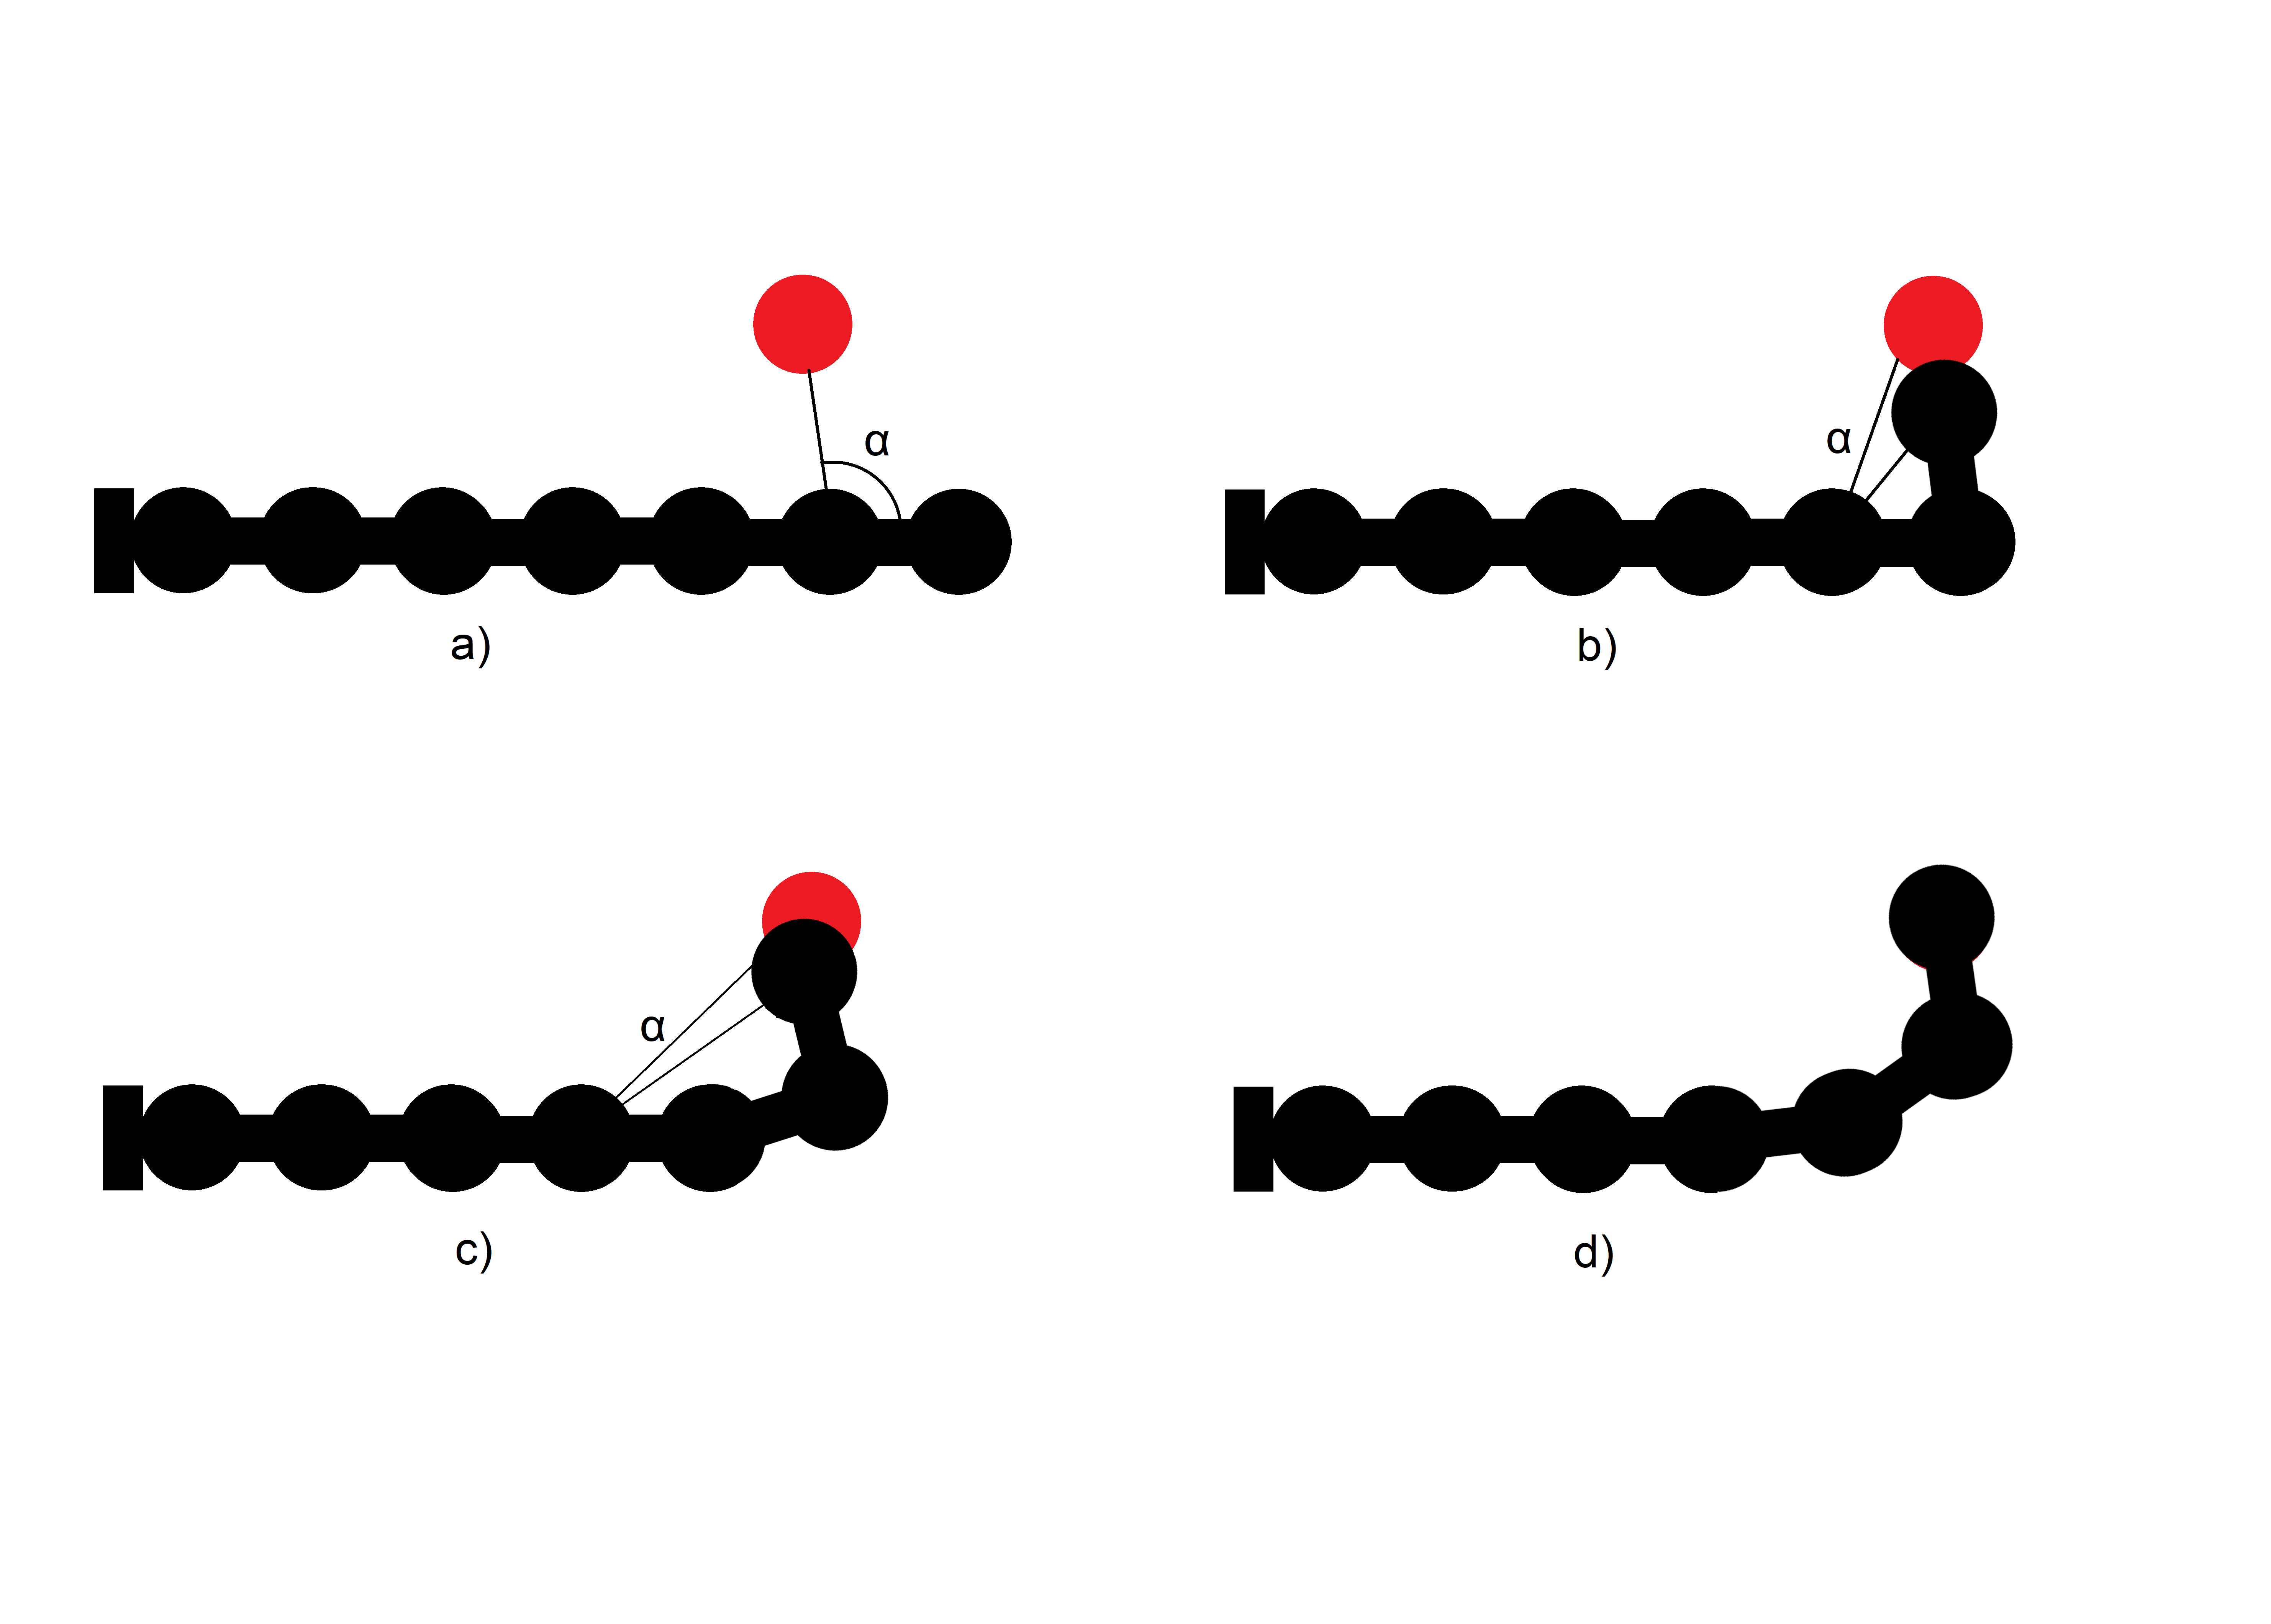
\includegraphics[width=0.35\textwidth]{ccd1.png}
    \caption{\\CCD algorithm~\cite{Ondika2021thesis}: The angles are repeatedly computed for each joint until a solution is found}
    \label{fig:ccd}
\end{wrapfigure}

The simplest of these methods is Cyclic Coordinate Descent (CCD)~\cite{ccd}. This algorithm iteratively goes through the joints of the manipulator, starting at the end effector, and turns each of them so that the distance to the target is locally minimized. Once it reaches the base, it starts iterating from the end again, until the end effector is close enough to the target (see Figure~\ref{fig:ccd}). This algorithm is fast, scales well, and in an unconstrained system, it always finds a solution, if one exists. However, the reached positions are very unnatural, which can lead to collisions with the environment, or even the manipulator itself. If we add obstacles or joint limits, the algorithm is also susceptible to local minima.

The state of the art method for inverse kinematics is the heuristic algorithm FABRIK:\ Forward and Backward Reaching Inverse Kinematics~\cite{fabrik}.
The algorithm consists of simple geometric computations, which are very fast. Just like the CCD method, it always finds a solution in unconstrained systems, and scales very well. Unlike CCD, it converges significantly quicker and computes natural poses.

\begin{figure}
    \centering
    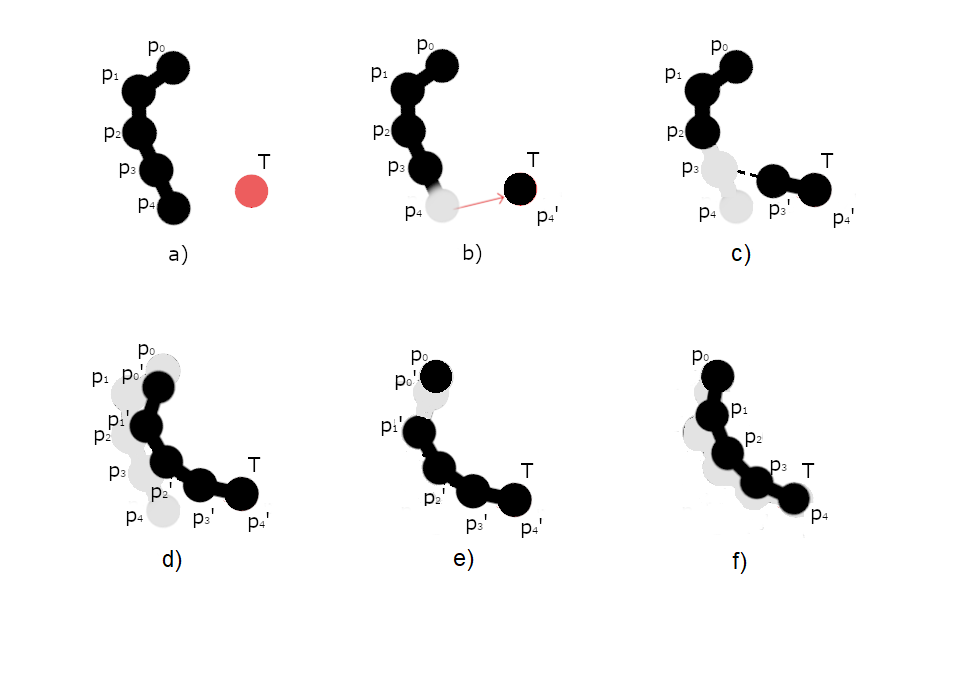
\includegraphics[width=0.8\textwidth]{fabrik.png}
    \caption[]{Fabrik algorithm~\cite{Ondika2021thesis}:
      \begin{enumerate*}
        \item[(a)] the initial position of the arm and the target
        \item[(b)] the end-effector $p_4$ is moved to the desired position
        \item[(c)] a vector between $p_3$ and the new $p_4$ is found, $p_3$ is repositioned along this line
        \item[(d)] arm after the forward reaching stage
        \item[(e)] the first point is moved to its initial position; the algorithm repeats itself in the other direction
        \item[(f)] final state; the base is in place and the target has been reached
       \end{enumerate*}
    }
    \label{fig:fab}
  \end{figure}

Rather than working with matrices or joint angles, the basic version of the algorithm calculates with points. As the name suggests, each iteration of the algorithm consists of two stages. In the first, forward reaching stage, the end-effector is moved to the desired target. Then, for each joint, the algorithm computes a line between the current and the next joint, which has already been moved. The current joint is moved along this line to the original distance between the two joints. Afterwards, the process is repeated for every joint, up until the base.

At this point, the algorithm has reached the target, but the immovable base may have been assigned a new position. Hence the algorithm is repeated, but this time it sets the base to the initial position and follows through with the algorithm all the way to the top. This forward and backward reaching is repeated until the base remains in its initial position and the end-effector reaches the target. Figure~\ref{fig:fab} illustrates the procedure.

The basic version of the algorithm is presented with rotational joints, but can be extended to any of the common types~\cite{fabrikConstraints}.

The FABRIK algorithm is very powerful and will serve us further, but note that inverse kinematics is just a subproblem of robot manipulator control. Even if we are able to compute the desired joint parameters for reaching a target, it remains unclear how to perform the motion from the initial position to the computed one. If there are obstacles in the environment, simply moving the joints to the computed positions is not possible.

\begin{figure}
\centering
\begin{subfigure}{.3\textwidth}
  \centering
  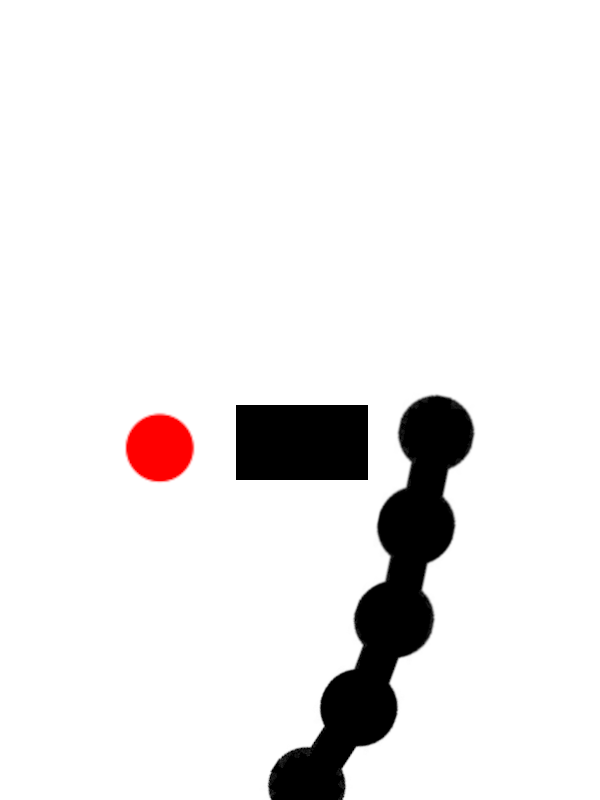
\includegraphics{IK_target.png}
  \caption{Initial position of the manipulator, a rigid obstacle and a target}
\end{subfigure}%
\begin{subfigure}{.3\textwidth}
  \centering
  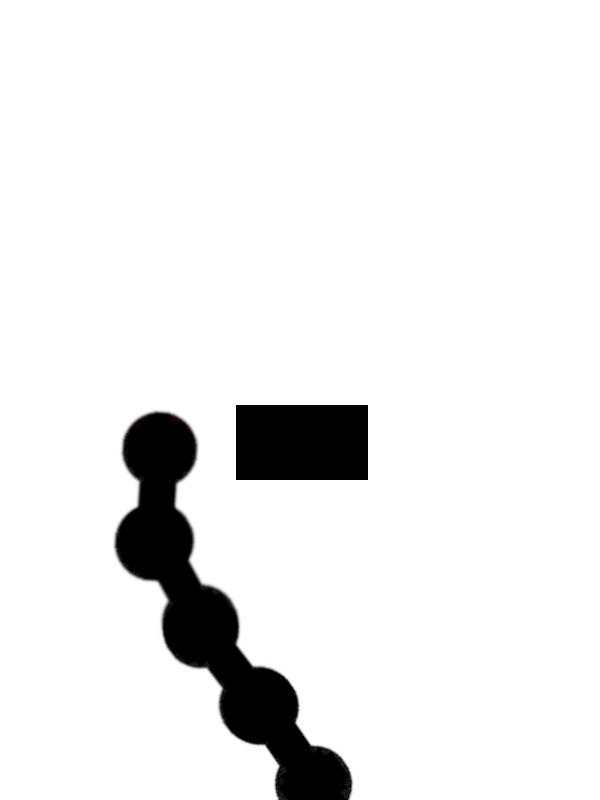
\includegraphics{IK_solution.png}
  \caption{A valid solution where the target is reached by the end effector}
\end{subfigure}%
\begin{subfigure}{.3\textwidth}
  \centering
  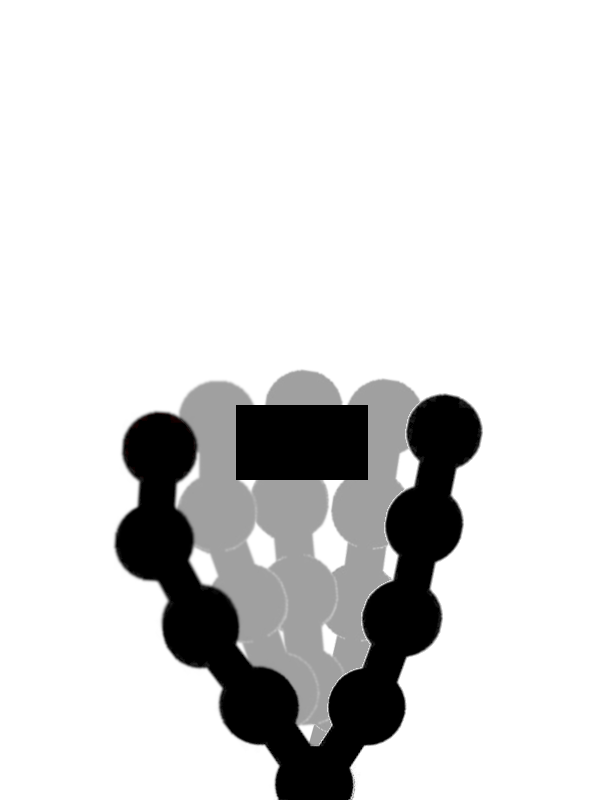
\includegraphics{IK_collision.png}
  \caption{Trying to rotate the joints would lead to a collision with the obstacle}
\end{subfigure}
\caption{A simple case where inverse kinematics is not enough to solve the motion planning problem.}\label{fig:ikcoll}
\end{figure}

\newpage
\section{The RoFI platform}

As technology progresses, research in robotics has moved on from single purpose manipulators used in factories. As of now, we are aiming towards more universal robots; robots that can be deployed in various situations, switch between different tasks, or even change shape. One of the interesting areas from the last few decades has been the concept of modular robots. Modular robots are small independent units, each with their own processors, batteries and usually a few joints. Each module can only perform basic tasks, but they have the ability to connect to each other and build more complex robots. Such a system is not as efficient at performing a single task as a single purpose industrial robot would be, but it has the potential to assemble different robots based on the task at hand and fulfill various roles.


\begin{figure}
    \centering
    
\includegraphics[width=1\textwidth]{rofi_platform.jpg}
  \caption{Logo of the RoFI platform~\cite{rofiPlatform}}
\end{figure}

There have been many research projects concerned with modular robots, each with their own approach to the task at hand. Some projects, such as Roombots~\cite{sprowitz_roombots_2010}, try to build solid structures that can disassemble once their task has been fulfilled. Roombots use sphere shaped modules along with passive blocks to assemble various pieces of furniture, which can be useful for saving space in small apartments or aiding people with disabilities with their daily tasks. Other systems, such as M-TRAN~\cite{mtran} or SMORES~\cite{smores}, try to build mobile robots from more universal modules. Such modules have a joint or two and can perform simple motion; by connecting to each other, they can build bigger robots and fulfill more complex tasks. The designs vary, and there hasn't been any clear winner in the field. An overview on the state of modular robotics can be found here~\cite{modular_survey}, but the field keeps evolving.

The RoFI platform~\cite{Mrázek2019thesis} is an open source modular robotics project developed at Masaryk University. The project is driven by students and consists of algorithmic research~\cite{Vozárová2019thesis, Zacek2021thesis, Nausova2022thesis, Ondika2021thesis, SMTReconfig}, development of hardware~\cite{Mrázek2019thesis, RoFICoM}, networking~\cite{Chlup2020thesis, Chlup2023thesis} and creating tooling for the development of the robots~\cite{Naušová2019thesis, Svoboda2020thesis}.

A robot within this platform, which we refer to as RoFIbot, is comprised of various modules. These can connect and disconnect based on the robot's needs, and allow it to change its overall shape.

\begin{wrapfigure}{r}{0.3\textwidth}
    \centering
    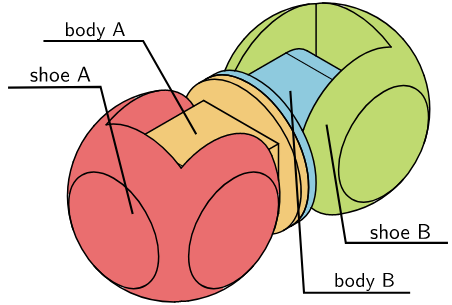
\includegraphics[width=0.3\textwidth]{um.png}
  \caption{Build of the universal module~\cite{rofiUm}}\label{fig:um}
\end{wrapfigure}

The basic building block of each robot within the platform is the universal module. It consists of two symmetrical bodies, wrapped in what we call shoes (see~\ref{fig:um}). The middle part of each module contains the hardware necessary for each module to function as an independent robot in itself. This includes rechargeable batteries to power the whole system, the main processor, which can run user programs, as well as coprocessors that manage firmware. The two bodies are connected to the main unit and perform motion and connection to the other modules.

\begin{wrapfigure}{l}{0.3\textwidth}
    \centering
    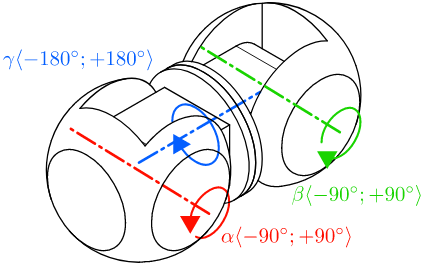
\includegraphics[width=0.3\textwidth]{um_joints.png}
  \caption{Rotation axes~\cite{rofiUm}}\label{fig:um_rot}
\end{wrapfigure}

Each body has a stepper motor that can turn from $-90$ to $90$ degrees. In our models, we refer to the joints as $\alpha$ and $\beta$. Per DH convention, the rotation is calculated as rotation around the $X$ axis with respect to the module's frame. What separates the design of RoFI modules from previous projects such as M-TRAN is the $\gamma$ joint, which allows unlimited rotation around the middle part of the robot, i.e.\ the $Z$ axis. The existence of this joint means that in combination with one of the other motors, the module can perform rotation in any direction, allowing it to perform more complex motions compared to its predecessors.

\begin{wrapfigure}{r}{0.3\textwidth}
    \centering
    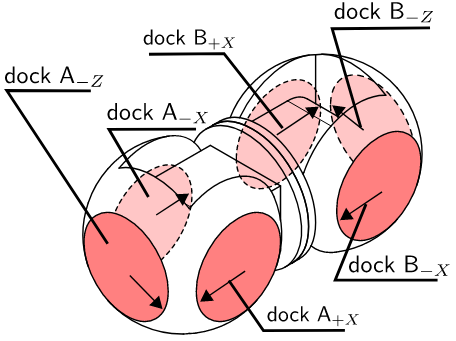
\includegraphics[width=0.3\textwidth]{um_connectors.png}
  \caption{RoFI connectors~\cite{rofiUm}}\label{fig:um_con}
\end{wrapfigure}

Each shoe has 3 connectors; we identify them via the shoe they're on and the direction they're facing with respect to the body. The connectors are genderless, which allows them to connect with any other connector within the plaform, and they can be retracted when not in use. Each connector is equipped with simple Lidar~\cite{Lidar} sensors. These perodically send out a laser that gets reflected off of nearby objects; this allows them to detect obstacles and estimate their distance based on how quickly the reflection returned. As a result, the modules don't have a full view of their environment, but each can locally detect nearby obstacles, as well as recognize whether there is another module they can connect to next to them.

Since each module has 3 degrees of freedom and the modules can be connected in various ways, the DoF of a RoFIbot rises very quickly with each module. If we wish to compute motion for the robot as a whole, traditional algorithms\footnote{Which are generally exponential with respect to the DoF, see the next chapter\ref{SotA}.} quickly become computationally infeasible. As one of the goals for this thesis is control of robotic arms comprised of such modules, a simulation within the RoFI platform will be used to demostrate our results.

  \chapter{State of the art}\label{SotA}

Tady:

- Motion planning as a whole, tj.\ začít s 2D robotem a vysvětlit obecné koncepty, abych se k tomu mohl vracet -- grafové algoritmy, APF, RRT.

- Generalizace A*, APF a RRT na robotická ramena, reference na aktuální články.

- Metody specifické pro robotická ramena, tj.\ hlavně optimalizační.

- Existující pokusy zkombinovat IK a motion planning, tj.\ podobné tomu co dělám já.

  \chapter{Extending FABRIK}

As we've established in earlier chapters, having a good algorithm for inverse kinematics can be a helpful tool for motion planning of robotic manipulators. It can be used in two ways:

\begin{itemize}
  \item Finding joint parameters that allow the manipulator to reach the target, and then looking for a way to reach the position with i.e. RRT.\ In this case, we don't mind if the IK algorithm is slow, since we are only computing it once. However, we want guarantees that a solution is found, if one exists.
  \item Finding a path with respect to the end effector with a different method, and using IK to find collision-free positions for the remaining joints. In this case, the priority is speed of computation, since it needs to be recomputed repeatedly.
\end{itemize}

In either case, the algorithm needs to be extended with a way to respect joint limits, and avoid collisions with surrounding obstacles. Since our aim is to be able to control manipulators with a high DoF, the latter option is more interesting for us.

\section{Adding joint limits to FABRIK}

When considering joint limits, computing the positions of points in space, as the original algorithm does (recall~\ref{fig:fab}), is no longer sufficient; we need to consider what kind of joint we are currently dealing with, and what its orientation in space is.

Instead of points in space, we can use a complete kinematic model of our robot. This model, per DH convention, contains information about what joints and bodies the robot consists of and what parameters the joints are currently at. As a result, the model calculates the corresponding matrices of each joint with respect to the rest of the world. Whenever a joint is moved, transformation matrices of the joints affected by this change are recomputed.

Since we want the kinematic model to stay connected, we can no longer easily disconnect the joint from the remainder of the configuration. Instead, a virtual copy of the manipulator is created and rooted at the target position.

[picture]

This way, the joints of the copy serve as points for the forward reaching stage, and the original joints serve as points for the backward reaching stage. Rather than detaching the current joint and moving it to the desired position, joints are moved at each step to minimize the distance, while respecting joint limits.

Finding the right joint parameters can be done by expressing the desired position in spherical coordinates~\cite{spherical}.

Spherical coordinates are an alternative way to describe points in space, different from the standard cartesian $x, y, z$ coordinates. In a spherical coordinate system, each point is uniquely described as $(r, \theta, \phi)$, where $r$ is the radial distance, which is any nonnegative number; $\theta$ is the azimuth angle, standardly ranging $0 \leq \theta < 2\pi$ and $\phi$ is the polar angle, standardly ranging $0 \leq \phi \leq \pi$. The limits are flexible, and we can change them to better match the possible joint rotations. For instance the polar angle can also range $-\pi \le \theta < \pi$, in which case the same points will be expressed slightly differently.

Using the inverse transformation matrix of our current joint, we can express the desired position in cartesian coordinates with respect to the joint. Then, the position can be converted to polar coordinates using the following equations:
\begin{equation}
  r = \sqrt{x^2 + y^2 + z^2}
\end{equation}
\begin{equation}
  \theta = \atantwo(\frac{x}{y})
\end{equation}

\begin{equation}
  \phi = \sin(\frac{z}{r})
\end{equation}

If the current joint allows for extension, we can extend or retract it to the correct radial distance. Rotations can be adjusted according to the two angles.

As the two stages alter iteratively, the two models converge to each other. Since the transformation matrices need to be recomputed repeatedly, the whole process is slower than the original algorithm, but gains several advantages.

\begin{itemize}
  \item The algorithm for forward and backward reaching is exactly the same, hence, it can be reused and the code is less sensitive to changes in the kinematic model.
  \item Both stages automatically respect the joint limits, since the model itself can validate the performed movements.
  \item Every movement of the original kinematic model can realistically be performed. We can ensure that our manipulator is always in a consistent state throughout the algorithm, which allows us to visualize the whole algorithm, generate intermediate steps for the purposes of animation, or stop the algorithm at any moment.
\end{itemize}

The most straightforward way to enforce that the joint limits are respected is to simply clamp the computed angles. If the algorithm computes an angle outside the range of the current joint,
the joint is instead set to the nearest feasible angle.

\begin{figure}[h]
    \centering
    \begin{minipage}{\textwidth}
        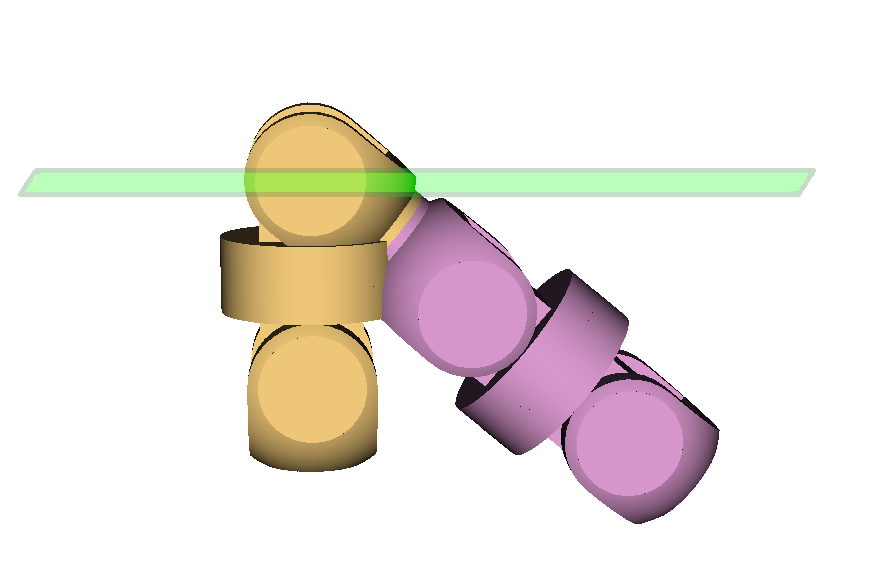
\includegraphics[width=.48\textwidth]{break_plane.png}
        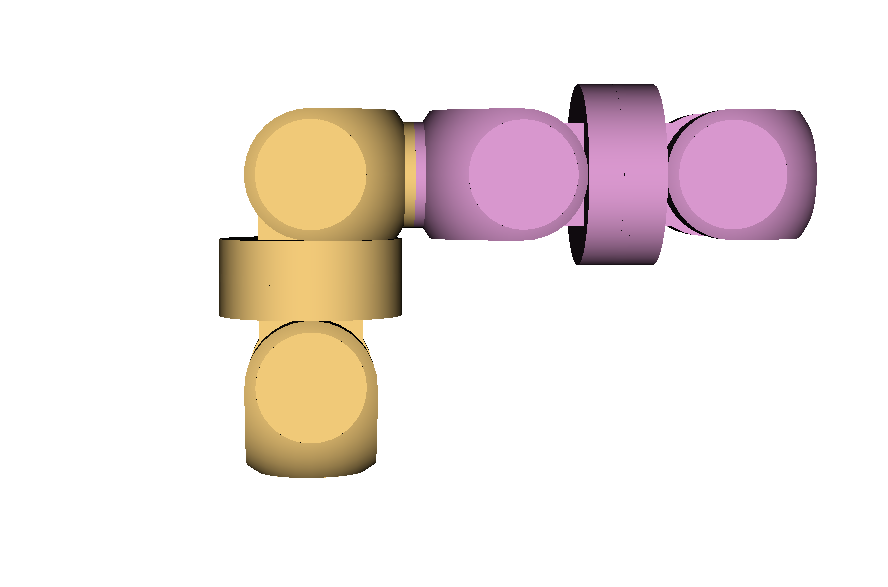
\includegraphics[width=.48\textwidth]{break_fixed.png}
    \end{minipage}
    \caption{The computed position violates the joint limit; the actual joint is clamped~\cite{Ondika2021thesis}.}\label{fig:break}
\end{figure}

While this limitation may prevent the algorithm from finishing in the current iteration, the other joints can make up for the limit and the manipulator is readjusted in the following iterations. In fact, as presented in~\cite{fabrik}, limitations on rotational joints can actually be helpful, in that more natural final poses are achieved.

The biggest problem we have to deal with comes when joints with only one degree of freedom are involved. Such joints can no longer rotate to an angle which minimizes the distance to the target joint, which means that we have to reason about the algorithm beyond the current joint for optimal results.

The optimal way to extend FABRIK to deal with this problem depends heavily on the build of the robot. Hence, in this part, the specifics of RoFI manipulators will be discussed; the core ideas may or may not translate to different manipulators.

Think back to the joints of the universal module (\ref{fig:um_rot}). When adapting the FABRIK algorithm to RoFI arms, we can treat each module as two joints. The joint between the two parts of a single module can only utilise the $\alpha$ or $\beta$ joint, hence, it is a simple rotational joint. As far as position of the next joint is concerned, the rotation of the $\gamma$ joint makes no difference. On the other hand, the joint between a universal module and the next component can utilise the $\gamma$ joint, and combine the two joints on the respective side to work as a ball joint and rotate in any direction. Passive modules or modules connected in a different direction can simply be viewed as a longer body between joints, and are not interesting for the algorithm.

The first idea that comes to mind may be to minimize the distance to the target joint position within the current limits. This is insufficient; if no special care is taken to account for joints that only have a single DoF, the manipulator will generally not reach the target.

The correct way to approach the problem is to align the one-dimensional joint in a way with the next target, so that only having one DoF is not limiting. Our implementation of FABRIK does exactly that: looking at the transformation created by the connection, the two DoF joint uses its mobility to place the next joint on the same plane as the target joint that follows it. As a result, the single DoF joint only needs to make a transformation in one plane, and the algorithm finds viable solutions to the constrained IK problem.

\begin{figure}[h]
    \centering
    \begin{minipage}{.6\textwidth}
        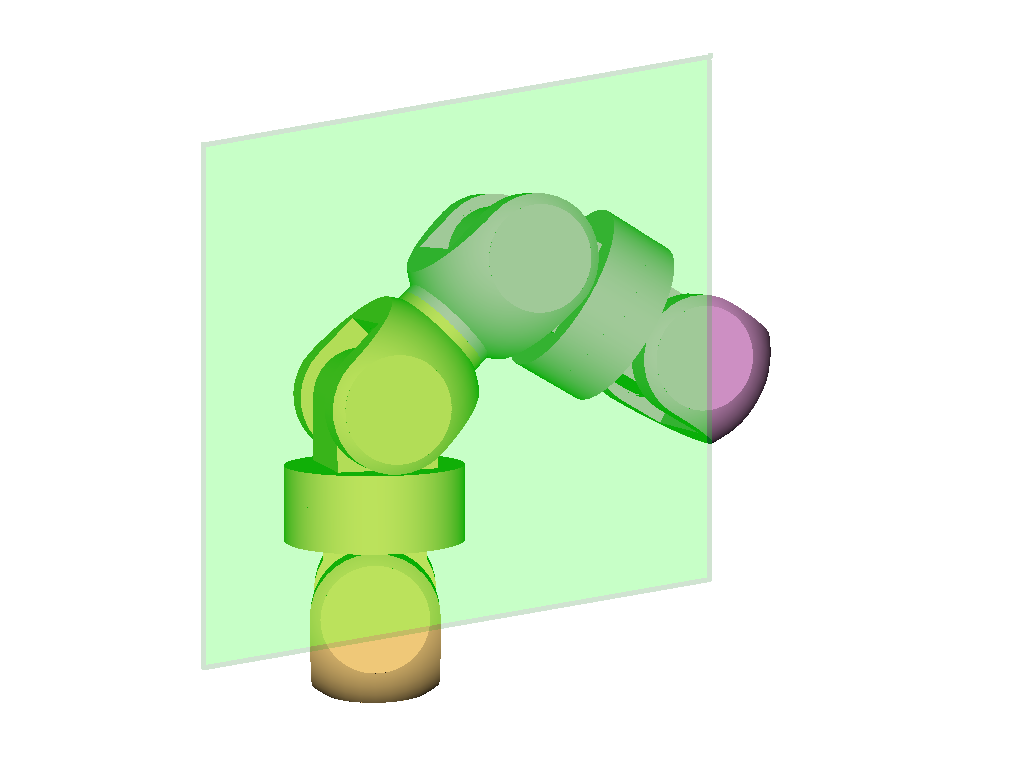
\includegraphics[width=\textwidth]{hinge_plane.png}
    \end{minipage}
    \caption{Visualization of the most common connection of modules: the first module is rotated so that the first joint of the second module lies in the target plane of the next joint~\cite{Ondika2021thesis}}\label{fig:hinge}
\end{figure}

Depending on the way the modules are connected, there are several cases that need to be dealt with in the implementation. A short summary:

\begin{itemize}
  \item Joint between parts of the same module: perform rotation along the X axis with respect to the current target
  \item Joint with Z-Z connection: perform rotation along the X axis with respect to the current target, rotation along the Z axis with respect to the following target
  \item Joint with Z-X connection: perform rotation along the X and Z axes with respect to the current target
  \item Joint with X-Z connection: perform rotation along Z with respect to the position of the current target, rotation along the X axis with respect to the following target
  \item Joint with X-X connection: perform rotation along the Z axis with respect to the current target
  \end{itemize}

Remeber that rotation along the joint's X axis is accomplished by the $\alpha$ and $\beta$ angles, while the rotation around Z corresponds to the $\gamma$ angle. The right angles are, as mentioned earlier, computed by fitting spherical coordinates to the possible movements of the joints: the azimuth angle (in radians) is clamped to $-\pi \le \theta < \pi$ to fit the $360\degree$ revolute Z joint, while the polar angle (in radians) is clamped to $-\frac{\pi}{2} \le \phi \le \frac{\pi}{2}$ to fit the $\left[-90\degree, 90\degree\right]$ X axis joint.

\section{Adding collision avoidance to FABRIK}

When discussing collision avoidance, the first question to ask is how to model the environment. Generally, we want to approximate objects in the workspace with simple geometric shapes: either polyhedra of choice, such as squares or pyramid shapes, or spheres. For simplicity and efficient representation, we shall choose the latter. Each joint of the manipulator shall be represented with a sphere\footnote{When considering RoFIbots, a single universal module can be modelled quite precisely with two adjacent spheres. With other types of robots, which may have longer bodies, rectangles or cylinders may be more suitable}. Without losing on generality, we can assume other objects in the workspace have also been approximated by the smallest sphere containing the entire shape.

For the moment, we will assume that the information about the workspace is complete; we know where all the objects are at the time we start the computation, and we have a complete model of the environment, created by a human or generated using an external camera.

One method for extending FABRIK with collision avoidance is presented here~\cite{fabrikAvoidance}. The authors propose that whenever a joint would be put in a position that causes a collision, the joint is put on a line between the current target and base of the arm, rather than the line between the current position and target. Then, if there is still a collision, a series of random rotations is used to avoid the obstacle.

If we were to compute IK only once, this method could prove useful. The method finds ways both around and between obstacles, and produces realistic poses. However, there are a few drawbacks:

\begin{itemize}
\item Since random rotations are used, there are no guarantees on the speed of convergence. As a result, as we can see from the authors' evaluation, the algorithm usually runs for around $0.1s$. We may be willing to wait that long once, but it is unimaginable to compute repeatedly.
\item Once again, no joint constraints are considered. When the current joint can only move in one plane, the initial guess of putting the joint as close to the base as possible is no longer well defined. In addition, random rotations in one direction may not lead to a solution due to hitting the joint limit, slowing the algorithm down even further.
\end{itemize}

In this thesis, a simpler approach to the collision avoidance problem within FABRIK is proposed.


During the forward reaching stage\footnote{Remember that in our extension, this moves the virtual copy of the manipulator, rooted in the target position.}, collisions are not checked. This allows the algorithm to find an approximate solution, but it is prone to collisions with surrounding objects.


During the backward reaching stage, the resulting position needs to be feasible. Hence, the new computed position for the joint is checked with the other objects in the workspace.

If the computed movement would cause a collision, a local limit is set on the current joint. A new joint rotation is computed within the limits set by nearby obstacles, and as a result, the manipulator gets as close to the desired position as possible, while avoiding a collision. The whole procedure is illustrated in Figure~\ref{fig:coll}.

\begin{figure}[h]
    \centering
    \begin{subfigure}{.24\textwidth}
      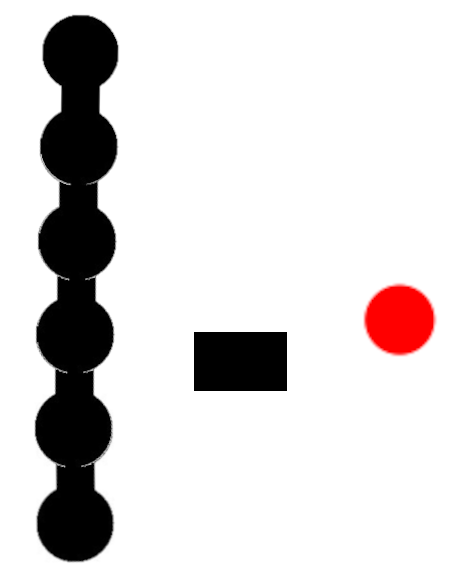
\includegraphics[width=0.9\textwidth]{coll_target.png}
      \caption{Initial position and target.}
    \end{subfigure}
    \begin{subfigure}{0.24\textwidth}
      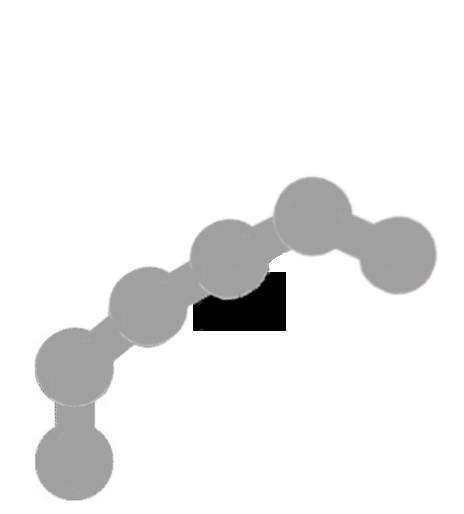
\includegraphics[width=0.9\textwidth]{coll_invalid.png}
      \caption{Solution from the first backward reaching stage.}
    \end{subfigure}
    \begin{subfigure}{.24\textwidth}
      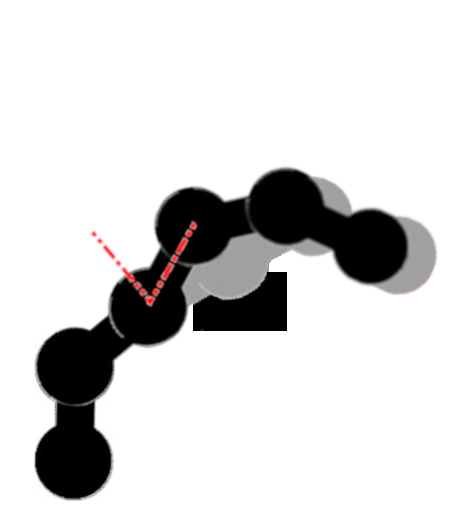
\includegraphics[width=0.9\textwidth]{coll_fixed.png}
      \caption{Collision is avoided by clamping the angle, but the target is not reached.}
    \end{subfigure}
    \begin{subfigure}{.24\textwidth}
      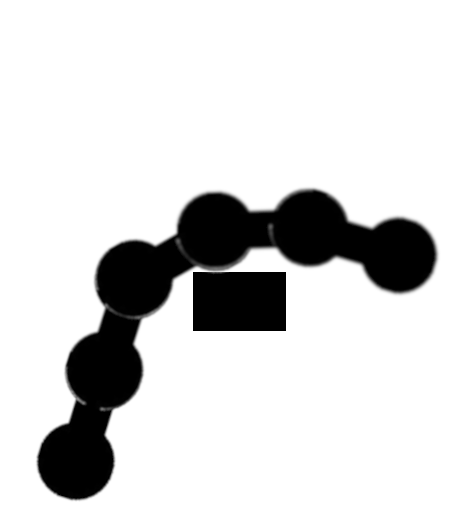
\includegraphics[width=0.9\textwidth]{coll_final.png}
      \caption{Final solution after a few iterations.}
    \end{subfigure}
    \caption{Illustration of FABRIK with simple collision avoidance.}\label{fig:coll}
\end{figure}
  
Note that compared to the aforementioned collision avoidance method, this one only works locally for each joint. As a result, it can get stuck in a local minimum, and not get over an obstacle. This is a disadvantage if we wanted to use it to immediately find a final solution; the algorithm could fail even though a solution exists. On the other hand, this behavior is desirable if we are using it to repeatedly compute incremental changes; the manipulator doesn't jump over obstacles when the actual movement is not directly possible. Additionally, the manipulator does not need complete knowledge of the environment, and we don't need to rely on randomness, which saves computational time and guarantees faster convergence.

As of now, we need to compare the new joint position with each other joint and each surrounding object in the workspace. Since other joints and obstacles are approximated with spheres, the collision check is very cheap: if the centers of two spheres are closer than the sum of their radii, the two spheres collide. However, checking every object is clearly asymptotically inefficient. Analog to doing lookup of strings or numbers in binary search trees, we would like to store our shapes in a structure that allows lookup with a logarithmic amount of comparisons.

A common structure for holding 3-dimensional information in robotics is the Octree~\cite{octree} -- this structure consists of squares, each of which is divident into 8 octants; subsquares of their parent. This structure allows easy lookup of data, but is not great for collision checking, since objects can span across various squares. In addition, modelling movement within an Octree can be difficult.

Hence, we opt for the data structure more commonly used in video games -- Axis Aligned Bounding Box Trees, AABB for short~\cite{aabb}. An AABB is a binary tree where shapes are stored in the leaves, and each inner node serves as the bounding box of its children. The bounding boxes are, as the name suggests, axis aligned -- we define them with standard $x, y, z$ dimensions and do not consider varying rotations. Unlike octrees, nodes in the AABB are of varying size, see Figure~\ref{fig:aabb}.

\begin{figure}[h]
  \centering
  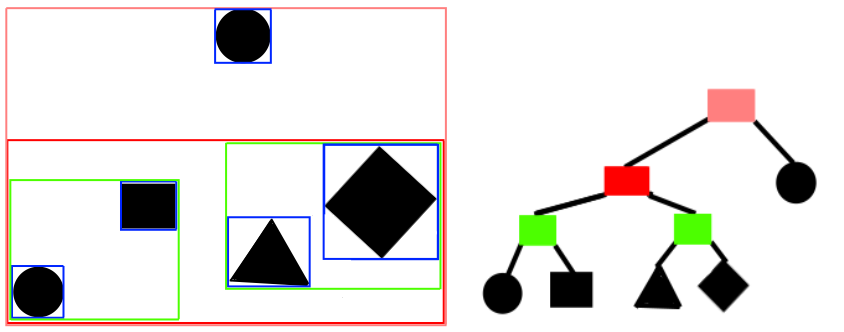
\includegraphics[width=0.8\textwidth]{aabb.png}
  \caption{Obstacles in space with the corresponding bounding boxes, and the inner structure of the AABB tree holding them.}\label{fig:aabb}
\end{figure}

The internal workings of an AABB are best explained using the actual operations. When the first shape is inserted into an AABB, a new node is created with a bounding box containing the shape. When inserting further shapes, the structure first chooses what leaf it shall become a sibling to, based on specified criteria.
Once a sibling has been chosen, the following operation proceeds:

\begin{enumerate}
\item Create a new parent node in place of the sibling leaf.
\item Make the sibling leaf a child of the new node.
\item Make the new leaf the other child of the new node.
\item Resize the parent node bounding box so that both shapes fit into it.
\item Recursively proceed to the root, increasing all the bounding boxes if necessary.
\end{enumerate}

\begin{figure}
  \centering
  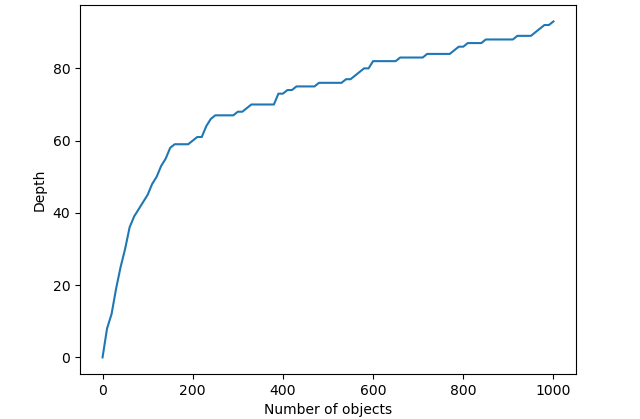
\includegraphics[width=0.6\textwidth]{aabb_depth.png}
  \caption{Graph of objects created at pseudorandom positions and the resulting depth of the tree.}\label{fig:aabb_depth}
\end{figure}

A common heuristic for choosing where to insert the new leaf is to descend the tree starting from the root, always choosing the child in that will lead to smaller resizing of the tree. When we perform random insertions, the tree balances itself out quite evenly (see Figure~\ref{fig:aabb_depth}).

The payoff for building the data structure in this way is efficient lookup. When we need to check if a shape would collide with any other shape already in the structure, we do not need to compare it to every leaf. Instead, collision lookup proceeds from the root and only enters nodes with bounding boxes that collide with our shape. If the shape does not collide with either of the bounding boxes, we know that it does not collide with the leaves either, as the leaf shapes are contained within the nodes by definition. If it does collide with a bounding box, we check for the children, potentially getting to leaf nodes. Then, finally, collision with the actual object is checked.

\begin{wrapfigure}{r}{0.4\textwidth}
  \centering
  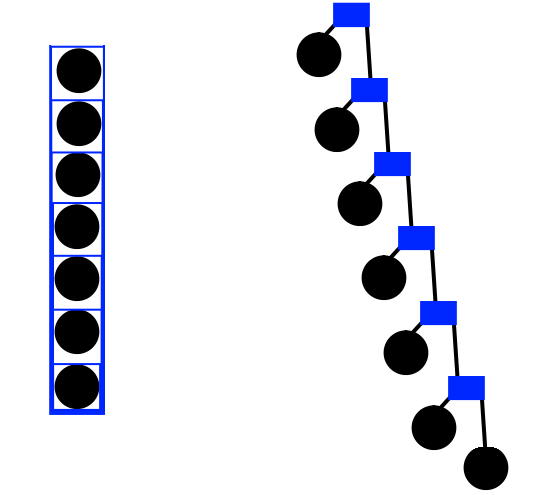
\includegraphics[width=0.4\textwidth]{degenerate.png}
  \caption{When objects are aligned and added one by one, a degenerate tree can be created.}
\end{wrapfigure}

In practice, the insertion heuristic performs well, and the \textit{expected} number of comparisons is significantly smaller than when trying to compare all the objects. However, the heuristic itself does not guarantee logarithmic depth; there is a case which leads to a degenerate tree. This tree can come to exist if all the objects are aligned and added to the tree starting from one end. Then, if we are checking collisions of an object close to the deepest leaf of our tree, the amount of comparisons is equal to the number of objects. This problem could be mitigated by adding balancing rotations to the tree, but in most cases, the extra work is unnecessary.

Now, how do we apply these trees to our problem? Assuming we already have a model of the environment, building the AABB is a simple matter of inserting each shape into it. To represent movement within an AABB, we need to erase the corresponding shape and then reinsert it at the new position.

Recall that in each backward iteration of FABRIK, we want to check if the current joint can be placed at the computed position. The invariant of our algorithm is that each joint has a corresponding sphere in the AABB, and the kinematic model of the manipulator has a pointer to it.

Therefore, we extend the backward FABRIK iterations by first erasing the joint leaves from the AABB. Then, when we compute a position for the joint, we check if it causes a collision with AABB lookup. If it does, we readjust it accordingly. When a reachable position for the joint is found, the joint is fixed for the remainder of the iteration, and the corresponding sphere is reinserted into the AABB. While it may seem that we've done a lot of unnecessary work, we can now guarantee that none of the joints will collide with other parts of the manipulator, or any static obstacle, without exhaustively checking all of them.

The difference may not be felt when all the obstacles are spheres, but it is particularly noticeable when we generalise obstacles to arbitrary shapes. Then, a collision check can be quite an expensive operation, and avoiding unnecessary checks with cheap bounding box comparisons can save a lot of computational time.

  \chapter{Path planning with respect to the end effector}

As of now, we have a fast inverse kinematics algorithm, which allows us to compute joint positions, given the \textit{end effector} position of the manipulator. If we can find a suitable path for the \textit{end effector} to follow, we can discretize it into small steps and use our extension of FABRIK to compute incremental changes along the path for the rest of the manipulator.

Although we have a myriad of algorithms to deal with the 3-dimensional path planning problem, the task is not as simple as our initial example of a robot that can move in any direction; we need to find paths that can be followed with the remainder of the manipulator.

This chapter goes through the process of designing such an algorithm for the task at hand.

\section{Grid based approach}

Recall that one of the successfull ways of applying this technique has been mentioned in~\cite{rrt_fabrik}, where the authors expand a RRT and compute FABRIK at every node. However, our extended FABRIK is too slow to compute for every point in the workspace; hence, we want to limit the amount of times we run the algorithm to lower hundreds.

Therefore, we want to find paths that lead to a solution with a high probability, and only compute FABRIK on points on this path. In case FABRIK fails on this path, for instance due to the manipulator being too short to get around an obstacle, we want to fall back and look for a different path.

Out of the three basic approaches, our go-to are the shortest path in a graph algorithms. As mentioned earlier, gradient based methods are not helpful due to the local minima problem and only generating a single possible path. Similarly, one of the weaknesses of the RRT algorithm is that it only finds a single path, and trying to generate edges between all possible nodes to find multiple paths would be computationally infeasible.

As a baseline for discretization of space, a grid based approach was tested out. This is not optimal for multiple reasons, but it is implementationally simple, allows us to analyze the procedure, and explore further extensions. Note that while the original Djikstra's algorithm works with weighted edges, in this case, we are assigning weights to vertices. Any edge that leads to a given vertex is treated as if it has the weight of the vertex during the shortest path algorithm.

Points on the grid were spaced out at half the size of a single joint, striking a balance between not generating too many points and making the shortest path algorithm too slow, and still being able to explore \textit{most} viable paths\footnote{This claim no longer holds if we consider many tiny obstacles, but the assumption that static objects are of comparable size to the joints of the manipulator is fairly reasonable. Spacing at half the joints' size means that if the manipulator fits in a space between obstacles, it will often be found.}.

The advantage of this representation is that we can weigh the points on the grid to influence which paths will be evaluated as optimal. We borrow the idea from the Artificial Potential Field algorithms, and give more weight to areas that surround an obstacle.

Points on the grid that are occupied by an obstacle are assigned an infinite weight, clearly no path can lead through them. In the area surrounding each obstacle, the weight will be high. Generally, we want the algorithm to choose paths further from obstacles, if possible. This follows the reasoning that we want to accomodate for the rest of the manipulator. If the path for the \textit{end effector} leads closely around obstacles, the chance that the remaining joints of the manipulator will fit is also lowered. However, while expensive, we want the paths close to obstacles to be evaluated as viable, since there may not be other options.

Each obstacle affects the surrounding area and raises the surrounding points on the grid based on how far they are. The total effect of obstacles is summed up; as a result, points between multiple obstacles are given a very high cost. A high cost between clusters of obstacles leads to the desired effect of preferring safer paths that avoid them altogether, though the path itself may be longer.

\begin{figure}
    \centering
    \begin{subfigure}{.3\textwidth}
      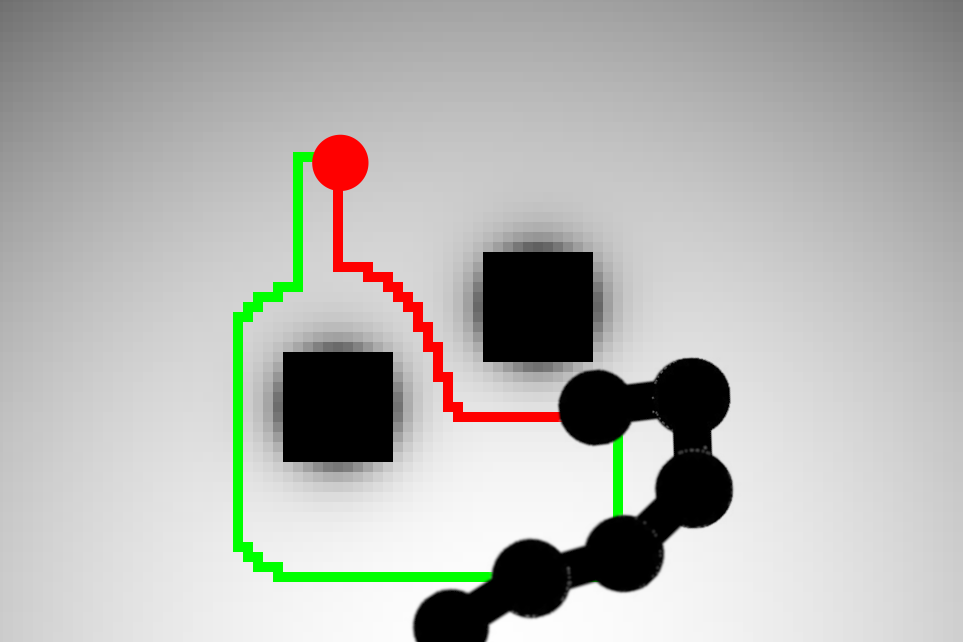
\includegraphics[width=0.99\textwidth]{manipulator_initial.png}
      \caption{Initial position of the manipulator, a target, and the first 2 paths found by the algorithm.}
    \end{subfigure}
    \begin{subfigure}{0.3\textwidth}
      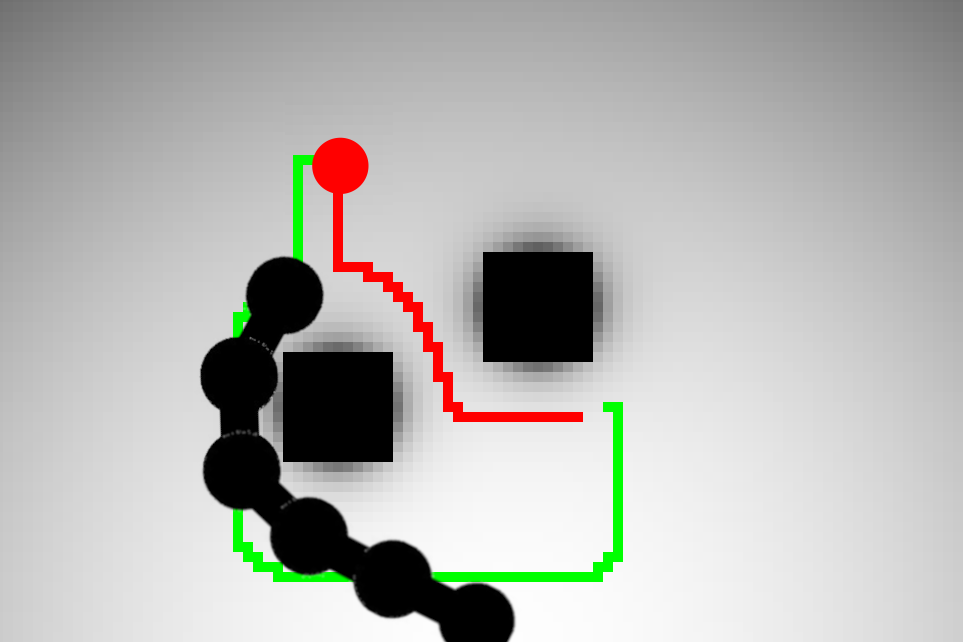
\includegraphics[width=0.99\textwidth]{manipulator_short.png}
      \caption{The careful path around obstacles does not lead to a solution, due to the manipulator being too short.}
    \end{subfigure}
    \begin{subfigure}{.3\textwidth}
      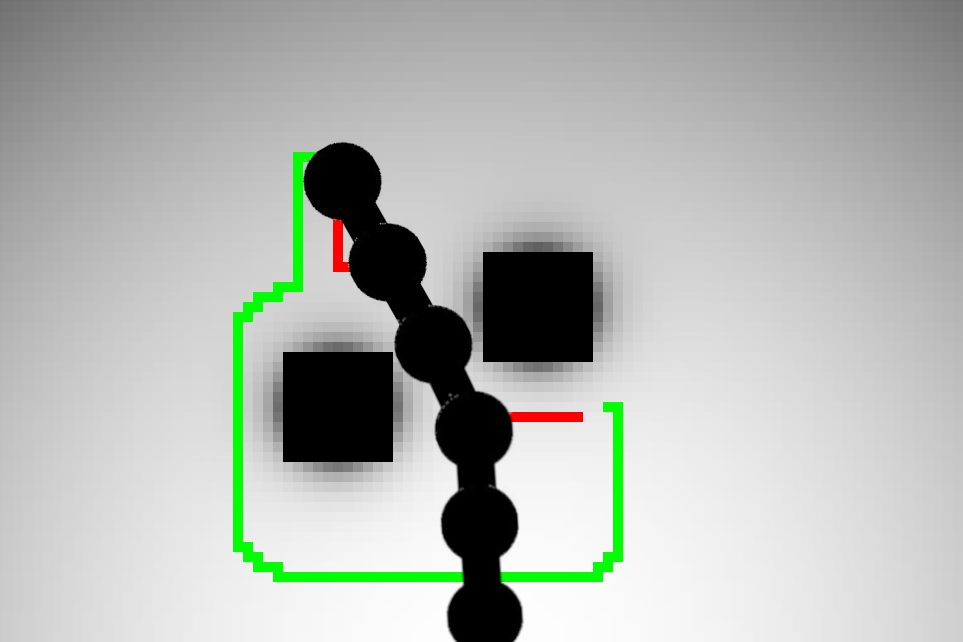
\includegraphics[width=0.99\textwidth]{manipulator_between.png}
      \caption{The viable path for the \textit{end effector} leads between the obstacles.}
    \end{subfigure}
    \caption{Illustration of the extended shortest path algorithm on a weighted grid. Black boxes represent obstacles, and the opacity of the background represents the cost of traversing over a given square.}\label{fig:paths}
\end{figure}

In effect, the algorithm works in the same fashion as APF, but does not suffer from local minima. If the first path we found is evaluated as wrong, the cost of points close to the found path is increased, and the algorithm looks for a new path in the modified graph. If, for instance, there are two obstacles and the only viable way to reach the target leads through them, paths around them may be evaluated as better at first. Trying to reproduce the path with FABRIK will fail due to the manipulator being too short, the cost near the found path is raised, and eventually the path between them is found. The idea is visualized in Figure~\ref{fig:paths}.

\begin{wrapfigure}{r}{0.4\textwidth}
  \centering
  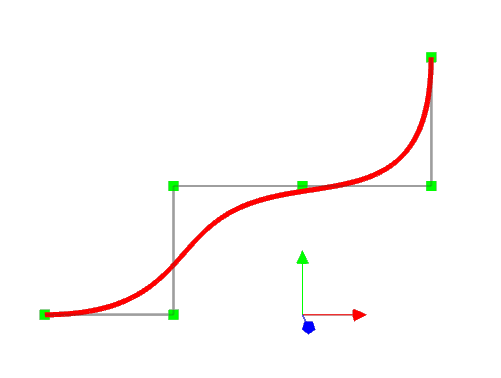
\includegraphics[width=0.4\textwidth]{nurbs_grid.png}
  \caption{B-splines can generate a smooth path from points on a grid (visualized using~\cite{nurbs_vis}).}
\end{wrapfigure}

The first obvious drawback of the algorithm is how rugged the resulting paths are. Instead of exactly following the found path and making unnecessary back and forth motion, we want to interpolate the points in a smooth way. Generating a smooth path from a set of points on the grid can be accomplished using B-splines~\cite{nurbs}.

B-splines, also known as basis splines, are piecewise polynomial functions used to generate smooth lines or shapes using a simple polynomial function and a set of control points.
To construct a B-spline, we need:

\begin{itemize}
\item A basis polynomial function given by its \textbf{order}. The order of the function determines how many nearby control points influence any the resulting points on the curve, and is always one more than the degree of the polynomial.
\item Sequence of \textbf{control points}. Control points determine the shape of the curve. Each point on the curve is determined as an interpolation between the nearby control points, using the sum of our basis functions for each of the points.
\item Sequence of \textbf{knots}. Knots are numbers in nondecreasing order, which determine where and how the control points affect the curve. The number of knots is always equal to the number of control points + the order of the curve. For trajectory generation, we can imagine the knot parameter as time. Then, we have a direct mapping of time to the position; knots specify by which control points the point will be influenced, and the ratio between the knot values specifies how much.
\end{itemize}

In the most common generalization of B-splines, Non-rational uniform B-splines (NURBS), each control point is also associated with a specific \textbf{weight}. When considering uniform points on a grid, we can just assign the same weight to each point.

Contrary to interpolating with polynomials directly, B-splines don't generally go directly through the control points. Going through a specific point can be achieved with a knot of a multiplicity equal to the order, which are commonly at the beginning and end of the curve. Since the curve order specifies how many control points influence each point, a lower curve order leads to curves closer to the control points, while a higher one can produce smoother paths overall.

\begin{figure}
  \centering
  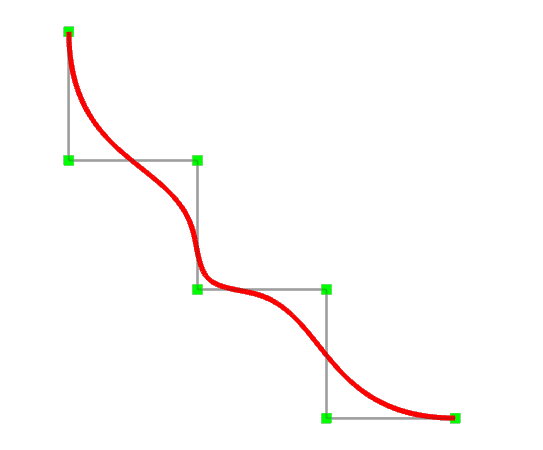
\includegraphics[width=0.5\textwidth]{nurbs_3.png}
  \caption{B-spline of order 4 with knots (0, 0, 0, 0, 0.4, 0.5, 0.6, 1, 1, 1, 1)}
\end{figure}

\begin{figure}
  \centering
  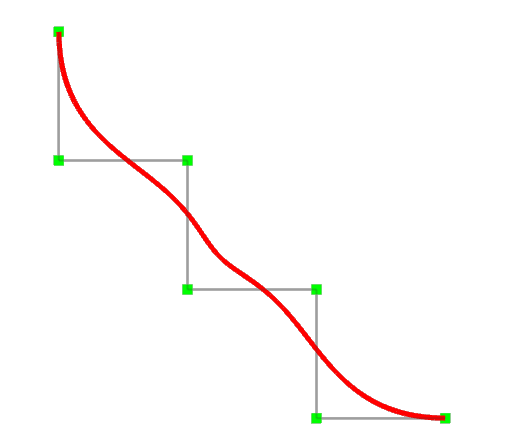
\includegraphics[width=0.5\textwidth]{nurbs_4.png}
  \caption{B-spline of order 5 with knots (0, 0, 0, 0, 0, 0.45, 0.55, 1, 1, 1, 1, 1)}
\end{figure}

To follow the curve with our inverse kinematics algorithm, we need to choose the size of our steps, get the value of the curve at the next time interval, and compute FABRIK starting at the current position. The only problem is that the curve only specifies the position, and the algorithm takes the entire transformation matrix as the input, including rotation. Hence, we need to look for ways to interpolate rotation as well.

In cases where the \textit{end effector} moves independently from the rest of the manipulator, Spherical linear interpolation (SLERP)~\cite{slerp} between the initial and target rotations is a suitable solution. The method uses quaternions to perform rotation at a constant velocity, resulting in a smooth motion.

Our case is a little different. In the case of RoFI manipulators, the rotation of the final module can influence how the entire manipulator needs to move, in order to accomodate for joint limits. Hence, we want to reach the target rotation as soon as possible. On the other hand, we need to consider that the target rotation may not be reachable immediately.

% This ensures that the subsequent sections are being included as root
% items in the bookmark structure of your PDF reader.
\bookmarksetup{startatroot}
\backmatter

  \begingroup
    \let\clearpage\relax
    \glsaddall
    \printglossary[type=\acronymtype]
    \newpage
    \printglossary
  \endgroup

  \printindex
  \printbibliography

\end{document}
